\label{sterowniki}
W rozdziale \ref{pierwsze_uruchomienie_aktualizacja_instalacja}: ,,Instalacja dodatkowych sterowników'' była opisywana metoda instalacji dodatkowych sterowników. Często w ten sposób instaluje się właśnie sterowniki do kart graficznych. Jednak skoro komputer wyświetla obraz jeszcze przed instalacją tych modułów, to znaczy, że jakieś sterowniki muszą już wcześniej być obecne w systemie. Zgadza się. W Ubuntu domyślnie są obecne sterowniki do niemalże każdej karty graficznej i rozwijane zgodnie z zasadami wolnego i otwartego oprogramowania. Spotykają się one z różną reakcją producentów sprzętu. Niektórzy oddają się im zupełnie i właśnie poprzez nie zapewniają oficjalne wsparcie dla Ubuntu, inni natomiast zupełnie je ignorują. Poza tymi sterownikami niektórzy producenci sprzętu dostarczają też na Ubuntu sterowniki oparte o zamknięty (własnościowy) kod źródłowy. Są to na ogół swegorodzaju porty ich odpowiedników z Windowsa, a dzięki temu zapewniają komplementarną z nimi wydajność i funkcjonalność. To te właśnie sterowniki możesz doinstalować na zasadach opisanych w rozdziale poświęconym dodatkowym sterownikom. W tym rozdziale dowiesz się więcej o tym z jakich sterowników powinieneś korzystać w twoim konkretnym przypadku.

\subsubsection{Identyfikacja karty graficznej i sterownika}
Żeby wiedzieć z jakich sterowników należy skorzystać, najpierw trzeba wiedzieć w jaki sprzęt wyposażony jest komputer. Część osób zapewne i bez żadnych dodatkowych procedur wie, jaką ma kartę graficzną, jednak żeby się upewnić należy w terminalu wpisać:

\begin{lstlisting}[language=bash]
lspci | grep VGA
\end{lstlisting}
\begin{itemize}
\item \textcolor{ubuntu_orange}{lspci} --- program wyświetlające urządzenia obecne w komputrze.
\item \textcolor{ubuntu_orange}{I} --- ,,rura'', ,,pipe'' przekierowanie wyjścia z jednego programu na wejście drugiego programu. 
\item \textcolor{ubuntu_orange}{grep} --- program wyszukujący wzorce.
\item \textcolor{ubuntu_orange}{VGA} --- szukany wzorzec, w tym wypadku szukamy urządzeń zgodnych ze standardem VGA (kart graficznych)
\end{itemize}

Wynik powyższej komendy zwróci producenta i nazwę karty graficznej, w jaką wyposażony jest komputer. Na przykład dla Nvidii:
\begin{lstlisting}[language=bash]
03:00.0 VGA compatible controller: NVIDIA Corporation G94 [GeForce 9600 GT] (rev a1)
\end{lstlisting}

Żeby dowiedzieć się z jakiego sterownika aktualnie korzysta twój komputer należy wpisać komendę:

\begin{lstlisting}[language=bash]
glxinfo | grep OpenGL
\end{lstlisting}
\begin{itemize}
\item \textcolor{ubuntu_orange}{glxinfo} --- program wyświetlające surowe informacje o aktualnie działającym sterowniku do karty graficznej.
\item \textcolor{ubuntu_orange}{I} --- ,,rura'', ,,pipe'' przekierowanie wyjścia z jednego programu na wejście drugiego programu. 
\item \textcolor{ubuntu_orange}{grep} --- program wyszukujący wzorce.
\item \textcolor{ubuntu_orange}{OpenGL} --- szukany wzorzec, w tym wypadku szukamy informacji o zgodności z bibliotekami OpenGL.
\end{itemize}

Uwaga! Powyższa komenda wymaga zainstalowania pakietu ,,mesa-utils''. Pakiet ten domyślnie doinstalowuje się wraz z \textcolor{ubuntu_orange}{ubuntu-restricted-extras}, którego instalacja była opisana w rozdziale \ref{ubuntu-restricted-extras}. Jeżeli już postąpiłeś zgodnie z tymi wytycznymi, to nie musisz wykonywać dodatkowej akcji, w przeciwnym przypadku odpowiedni pakiet można doinstalować komendą:
\begin{lstlisting}[language=bash]
sudo apt-get install mesa-utils
\end{lstlisting}
\begin{itemize}
\item \textcolor{ubuntu_orange}{sudo} --- wykonuje dalsze polecenia z uprawieniami administratora systemu.
\item \textcolor{ubuntu_orange}{apt-get} --- program do zarządzania zainstalowanym oprogramowaniem.
\item \textcolor{ubuntu_orange}{install} --- informujesz apt, że chcesz zainstalować paczkę z oprogramowaniem.
\item \textcolor{ubuntu_orange}{mesa-utils} --- nazwa paczki do zainstalowania.
\end{itemize}

\subsubsection{Intel}
Karty graficzne produkowane przez Intela to najprostszy przypadek w Ubuntu. Intel oficjalnie rozwija jedynie otwarte sterowniki, które już są obecne zaraz po instalacji systemu. Żadna dodatkowa akcja nie jest wymagana przez użytkownika. Można dodatkowo zainstalować dwa pakiety, aby zapewnić akcelerację sprzetową dla dekodowania filmów:

\begin{lstlisting}[language=bash]
sudo apt-get install i965-va-driver vainfo
\end{lstlisting}

\subsubsection{nVidia}
Po przeciwnym biegunie jest natomiast nVidia. Ten producent prawie zupełnie ignoruje otwarte sterowniki, ale za to dostarcza zamkniętych modułów, które są wysokiej jakości. Zamknięte moduły instaluje się zgodnie z rozdziałem \ref{pierwsze_uruchomienie_aktualizacja_instalacja}: ,,Instalacja dodatkowych sterowników''. 

\begin{center}
	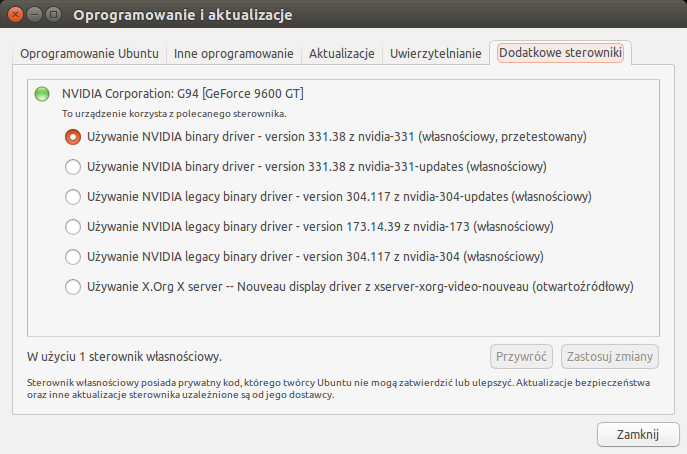
\includegraphics[width=\linewidth]{images/pierwsze_uruchomienie_driver2.png}
\end{center}

Dla odpowiednich kart graficznych należy zainstalować sterowniki o wskazanych numerach:
\begin{itemize}
\item Sterownik 331.x dla kart GeForce 8000 i nowszych
\item Sterownik 304.x dla kart 6000 -- 7000
\item Sterownik 173.x dla kart GeForce 5 (FX)
\item Sterownik 96.x dla kart GeForce 4 i starsze
\end{itemize}

Oprogramowanie do instalowania dodatkowych sterowników powinno poprawnie zidentyfikować i zaproponować wersję do instalacji.
Akcelerację wideo poprzez VDPAU można doinstalować poleceniem:

\begin{lstlisting}[language=bash]
sudo apt-get install libvdpau1 vdpauinfo
\end{lstlisting}

Jeśli twój komputer to laptop z układem NVidia Optimus, a system nie rozpoznał tego układu, to może zajść potrzeba ręcznej instalacji pakietu nvidia-prime. 

\begin{lstlisting}[language=bash]
sudo apt-get nvidia-prime
\end{lstlisting}

\noindent Możliwość przełączania układu graficznego znajduje się w panelu ustwień \textcolor{ubuntu_orange}{nvidia-settings}.

Gdyby pakiet nvidia-prime nie zdawał egzaminu, można go odinstalować i w jego miejsce zainstalować Bumblebee. Ten program wyłącza dyskretną kartę NVidii, jednocześnie umożliwiając jej włączenie wtedy, gdy jest potrzebna.
Po wcześniejszym odinstalowaniu nvidia-prime Bumblebee można zainstalować poleceniem:

\begin{lstlisting}[language=bash]
sudo apt-get install bumblebee bumblebee-nvidia
\end{lstlisting}

\subsubsection{AMD}
AMD jest czymś między Intelem, a nVidią. Z jednej strony dostarcza zamknięte sterowniki (ale tylko dla najnowszych kart graficznych), z drugiej strony rozwijają otwarte sterowniki, które wspierają starsze modele. W związku z tym jeżeli jesteś użytkownikiem karty graficznej AMD Radeon HD 5000 lub nowszej powinieneś zainstalować zamknięte sterowniki zgodnie z procedurą opisaną w rozdziale \ref{pierwsze_uruchomienie_aktualizacja_instalacja}: ,,Instalacja dodatkowych sterowników''. W przypadku posiadania starszej karty graficznej powinieneś pozostać na otwartych sterownikach.

\begin{center}
	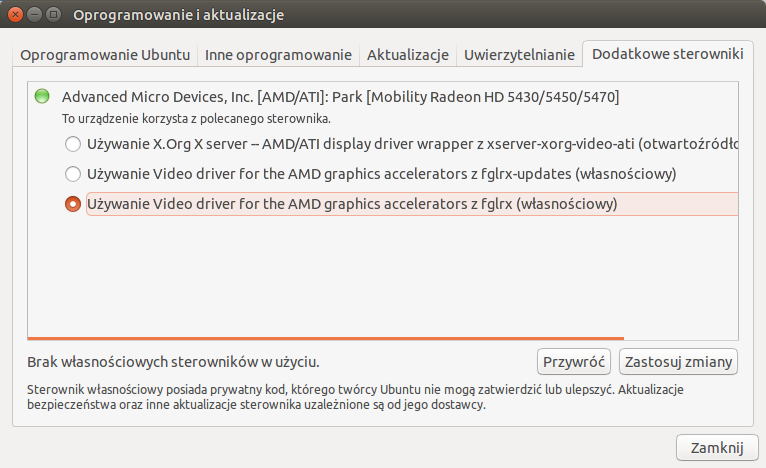
\includegraphics[width=\linewidth]{images/sterowniki_AMD.png}
\end{center}

W tym drugim wypadku można zapewnić akcelerację wideo poprzez VDPAU instalując pakiety poleceniem:
\begin{lstlisting}[language=bash]
sudo apt-get install libvdpau1 vdpauinfo mesa-vdpau-drivers
\end{lstlisting}

Posiadacze hybrydowych układów AMD powinni zainstalować paczki fglrx oraz fglrx-pxpress:

\begin{lstlisting}[language=bash]
sudo apt-get install fglrx fglrx-pxpress
\end{lstlisting}